% vim: ft=tex
%!TEX root=../ast2016.tex

% GRAPHIC: This is the bar chart of the number of mutants that each technique ran during mutation analysis
% NOTE: This graph was removed due to space constraints, it can be summarized in the text, I think.
% BOXPLOT input
%!TEX root=ast2016.tex

\begin{figure*}[t]
  \centering
  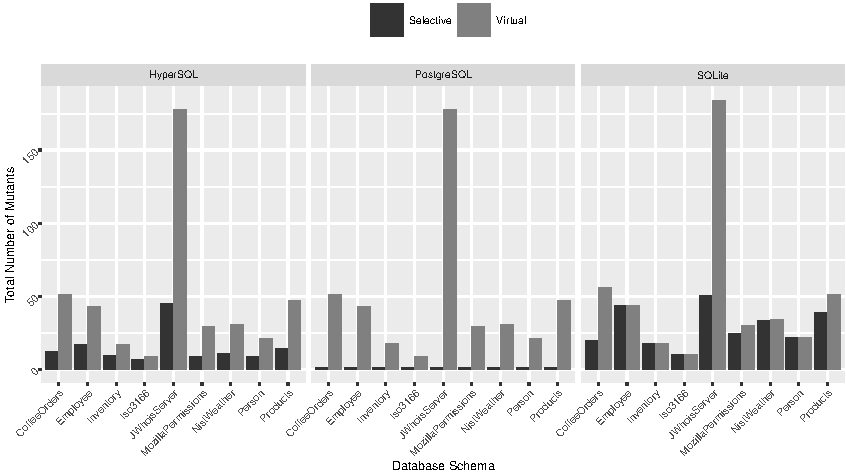
\includegraphics[scale=1.0]{graphics/graphic_barplot_schema_mutantcount_vm_tcm.pdf}
  \caption{Bar plot of the mutant count for both the virtual and time-constrained mutation analysis techniques.}
  \label{fig:graphic_barplot_schema_mutantcount_vm_tcm}

  {\small \justifying{ \noindent In this plot the height of the bar corresponds to the number of mutants subject to
      analysis by the virtual and time-constrained methods; this count is reported for all of the chosen relational
      schemas and the three database management systems. Since the time-constrained technique employs randomness to
      select mutants that can be run within a specified time limit, the height of a light grey bar is the average across
      a total of thirty runs; virtual mutation analysis is deterministic and thus the height of the dark grey bar is a
      direct count. } \par}

\end{figure*}


\inlineheading{Virtual and Time-Constrained Mutation} Since the experiments revealed that \vma~is faster than the \Original~one in $22$ out of the $27$ studied configurations --- and competitive with the DBMS-based method in the other $5$ --- it is useful to ascertain whether the presented technique might yield more accurate mutation scores in some circumstances. To this end, Figure~\ref{fig:graphic_bwplot_schema_mutationscore_vm_tcm} presents the mutation score of both the virtual approach and a time-limited analysis in which \Original~randomly analyses mutants for as long as virtual. These box plots show that the time-constrained technique results in mutation scores that are often highly variable. This result can be attributed to randomness inherent in running mutation analysis under a strict time limit that will not permit the examination of every mutant.
%
% PSM: TODO-FOR-GREG - nope not true! (As discussed on Slack)
For instance, the noticeable variability in \mbox{mutation} score when the Person schema is run on \Postgres~is due to the possibility of not finishing the analysis of the first mutant. The bar chart in Figure~\ref{fig:graphic_barplot_schema_mutantcount_vm_tcm} confirms this explanation by revealing that the time-constrained approach rarely analyses as many mutants as does virtual, especially for large schemas like JWhoisServer.

Bearing in mind that the virtual method produces mutation scores that are always equal to those achieved by the standard technique, it is also important to observe that time-constrained mutation analysis leads to overly high mutation scores.  Yet, at least for the \HyperSQL~and \SQLite~DBMSs, the box plots in Figure~\ref{fig:graphic_bwplot_schema_mutationscore_vm_tcm} suggest that the mutation scores are roughly similar for \vma~and the time-constrained method. To rigorously establish this correlation, we calculated Kendall's \taub~for the two techniques on each of the DBMSs, arriving at the values of $0.561$ (moderate), $0.132$ (low) and $0.756$ (high) for \HyperSQL, \PostgreSQL and \sqlite, respectively. These correlations suggest that virtual mutation is the best option when highly accurate scores are needed and there is limited time for mutation analysis of a database schema.

